\section{Modular functions}

We devote the last section of this thesis to the visualization of modular functions. The theory of modular functions is a branch of complex analysis whose importance and beauty lies most notably in its connections to number theory. We will however not dive deeply into this theory. Instead we will content ourselves with depicting graphs of certain selected modular functions, enjoying their visual aesthetics and reading off some of its properties, like zeros and poles as well as their order. Unfortunately such illustrations of modular functions are rarely found in literature. Therefore this section should be considered as complementary material to more comprehensive treatments of modular functions given for example in \Klein{}, \Lehner{} or \Schoeneberg{}.

\index{Meromorphic function}
Modular functions are meromorphic maps (\ie maps which are holomorphic\footnote{Holomorphic functions are also frequently called ``analytic''.} except for isolated poles, or in other words, maps which can be represented as quotient of two holomorphic functions) which are defined on the upper half-plane and which are invariant under the transformations of the modular group.

\begin{definition}[Modular function]
Let the upper halfplane $\mathcal{H}$ and the extended upper halfplane $\EU$ be defined as in (\ref{eqn_Upperhalfplane}) and (\ref{eqn_ExtUpperhalfplane}) respectively.
A map $f : \EU \to \EC$ is called a \emph{modular function}, if it satisfies the following conditions:
\begin{enumerate}[\quad(i)]
\item $f$ is meromorphic on the upper half-plane $\mathcal{H}$.
\item On $\EU$ we have $f = f \circ A$ for all $A \in \PSL{\Z}$.
\item There is a constant $C \ge 0$ such that $f$ has a series expansion of the form
\begin{equation*}
f(z) = \sum_{k \ge k_0} a_k \exp(2 \pi \ii k z),
\end{equation*}
with $k_0 \in \Z$, $a_k \in \C$, $a_{k_0} \ne 0$, which converges for all $z \in \mathcal{H}$ with $\Im{z} > C$. Moreover, 
\begin{equation*}
f(\infty) = \begin{cases}
0 & \text{if } k_0 > 0,\\
a_0 & \text{if } k_0 = 0,\\
\infty & \text{if } k_0 < 0.
\end{cases}
\end{equation*}
\end{enumerate}
\end{definition}

\begin{remark}For the proof that modular functions indeed exist we refer to \Schoeneberg{}, Chapter II, �3.
\end{remark}

\index{Absolute modular invariant}
\index{Klein's complete invariant}
A modular function of essential importance is the $J$ function, also known as the \emph{absolute modular invariant} or \emph{Klein's complete invariant}. One of its important properties is, that on the fundamental domain $\FunDom$ it takes on each value in $\EC$ exactly once. In other words, $J$ can be considered as bijective map from $\FunDom$ to $\EC$. 

In order to discuss this one-to-one mapping between $\FunDom$ and $\EC$ under $J$, let us denote the boundary arcs of $\FunDom$ again by $a,b,c$ and $d$, as in Figure~\ref{fig_PSL2FunDom}. Moreover, denote by $e := \setdef{\lambda \ii}{\lambda \ge 1} \cup \{\infty\}$ the arc which splits $\FunDom$ into two symmetric havles, \ie two open connected components. Let us denote these open sets by $\FunDom_\text{left}$ and $\FunDom_\text{right}$ respectively. For the special boundary points $\ii$, $\rho$ and $\infty$ we have
\begin{equation*}
J(\ii) = 1, \quad J(\rho) = 0, \quad J(\infty) = \infty.
\end{equation*}
Moreover, the following mappings of sets are all injective:
\begin{itemize}
\item The left boundary arc $a$ and the right boundary arc $b$ of $\FunDom$ are both mapped to the set $\overline{\R}_{\le 0} := \setdef{z \in \R}{z \le 0} \cup \{\infty\}$:
\begin{equation*}
J(a) = J(b) = \overline{\R}_{\le 0}.
\end{equation*}
\item The boundary arcs $c$ and $d$ of $\FunDom$ are both mapped to the interval $[0,1]$:
\begin{equation*}
J(c) = J(d) = [0,1].
\end{equation*}
\item The ``symmetry arc'' $e$ is mapped to $\overline{\R}_{\ge 1} := \setdef{z \in \R}{z \ge 1} \cup \{\infty\}$:
\begin{equation*}
J(e) = \overline{\R}_{\ge 1}. 
\end{equation*}
\end{itemize}
In particular, the boundaries of $\FunDom_\text{left}$ and $\FunDom_\text{right}$ are both injectively mapped to $\R \cup \{\infty\}$. 
Finally, the images of $\FunDom_\text{left}$ and $\FunDom_\text{right}$ under $J$ are exactly the upper and lower half-plane:
\begin{equation*}
J(\FunDom_\text{left}) = \mathcal{H} \quad\text{and}\quad
J(\FunDom_\text{right}) = -\mathcal{H}.
\end{equation*}

Unfortunately, plotting the function graph of $J$, or more generally the function graph of any map $f: \EC \to \EC$ is not directly possible, as it is in fact a 4-dimensional object.\footnote{It involves two dimensions for real and imaginary part of the function argument and two more dimensions for real and imaginary part of the function value.} However there is a simple idea for getting around this problem: We assign each $z \in \EC$ a certain color $\col{z}$ and obtain a picture of $f$ by dying each point $z$ on the complex plane in the color $\col{f(z)}$. Our choice of the color coding is quite simple: 
\begin{itemize}
\item The tone of the color $\col{z}$ encodes the complex argument of $z$:\\
\begin{tabular}{rlccccc}
Red &($\arg{z} = 0$) &$\to$& Orange &$\to$& Yellow &$\to$ \\
Green &($\arg{z} = \half{\pi}$) &$\to$& Turquoise &$\to$ \\
Cyan &($\arg{z} = \pi$) &$\to$& Blue &$\to$\\
Violet &($\arg{z} = -\half{\pi}$) &$\to$& Magenta &$\to$& Red (again).
\end{tabular}
\item The saturation and brightness of the color $\col{z}$ encodes the absolute value of $z$. For this purpose, we use the continuous map 
\begin{equation*}
b(r) := \begin{cases}
0 & \text{if } r = 0,\\
\reci{\pi}\arctan(\ln r)  + \reci{2} & \text{if } r \in (0,\infty),\\
1 & \text{if } r = \infty
\end{cases}
\end{equation*}
to first bring $\abs{z}$ to the interval $[0,1]$. Then we define the saturation of $\col{z}$ as $1 - b(\abs{z})^2$ and its brightness as $1 - (1 - b(\abs{z})^2)$. This means that $\col{z}$ changes gradually from a perfect black (if $z = 0$) to a perfect white ($z = \infty$) as absolute value of $z$ grows.
\end{itemize}
\begin{figure}
\centering
\includegraphics[width=0.8\textwidth]{figures/klein-j}
\caption{The composition of the Klein modular invariant function and the inverse modified Cayley transform $j \circ \inv{\ModCayley}$.}
\label{fig_KleinJ}
\end{figure}


\begin{figure}
\centering
\begin{tabular}{c c c}
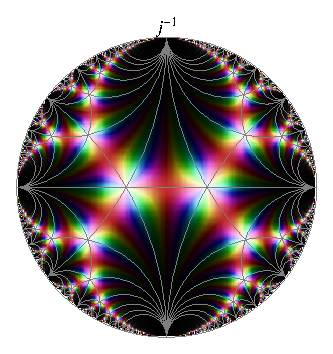
\includegraphics[width=0.45\textwidth]{figures/klein-jinv} & \quad &
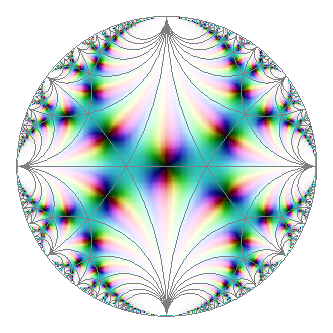
\includegraphics[width=0.45\textwidth]{figures/klein-jm1} \\
\\
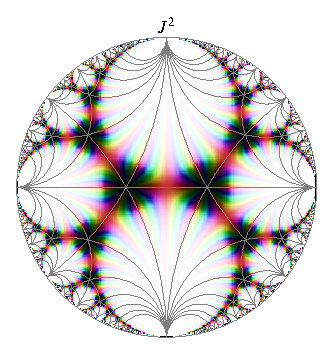
\includegraphics[width=0.45\textwidth]{figures/klein-jsqr} & \quad &
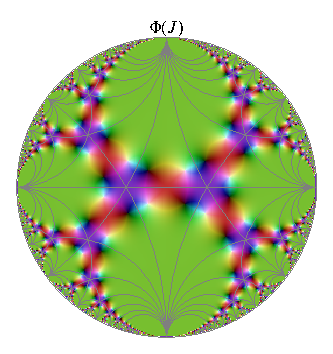
\includegraphics[width=0.45\textwidth]{figures/klein-j-mod-cayley}
\end{tabular}
\caption{The composition of the Klein modular invariant function and the inverse modified Cayley transform $j \circ \inv{\ModCayley}$.}
\label{fig_FunctionsOfJ}
\end{figure}

\begin{figure}
\centering
\includegraphics[width=0.8\textwidth]{figures/klein-jfib-large}
\caption{The composition of the Klein modular invariant function and the inverse modified Cayley transform $j \circ \inv{\ModCayley}$.}
\label{fig_KleinJFib}
\end{figure}
